\documentclass{beamer}

\mode<presentation> {

\usetheme{Madrid}
\usecolortheme{dolphin}

}

\usepackage{graphicx}
\usepackage{booktabs}
\usepackage{physics}

%----------------------------------------------------------------------------------------
%	TITLE PAGE
%----------------------------------------------------------------------------------------

\title[MC methods for PDEs]{Monte Carlo methods for Solving PDEs\\Computational Physics Final Project}

\author{Yucheng Zhang}
\institute[Physics @ NYU]
{
Department of Physics, New York University \\
\medskip
\textit{yz4035@nyu.edu}
}
\date{\today}

\begin{document}

\begin{frame}
\titlepage
\end{frame}

\begin{frame}
\frametitle{Overview}
\tableofcontents
\end{frame}

%----------------------------------------------------------------------------------------
%	PRESENTATION SLIDES
%----------------------------------------------------------------------------------------

\section{Introduction}

%------------------------------------------------

\subsection{Laplace's Equation with Dirichlet Boundary Condition}

\begin{frame}
\frametitle{Laplace's Equation with Dirichlet Boundary Condition}
\begin{itemize}
\item
\begin{equation}
    \begin{split}
        &\nabla^2 u = 0 \qquad \text{on}\quad G, \\
        &u = f(x) \qquad \text{on}\quad \partial G.
    \end{split}
\end{equation}
\item
Discrete form with centered finite difference approximation,
\begin{equation}
    u_{i,j} = \frac{1}{4} \qty(u_{i+1,j}+u_{i-1,j}+u_{i,j+1}+u_{i,j-1}).
\end{equation}
\begin{figure}[htbp]
    \centering
    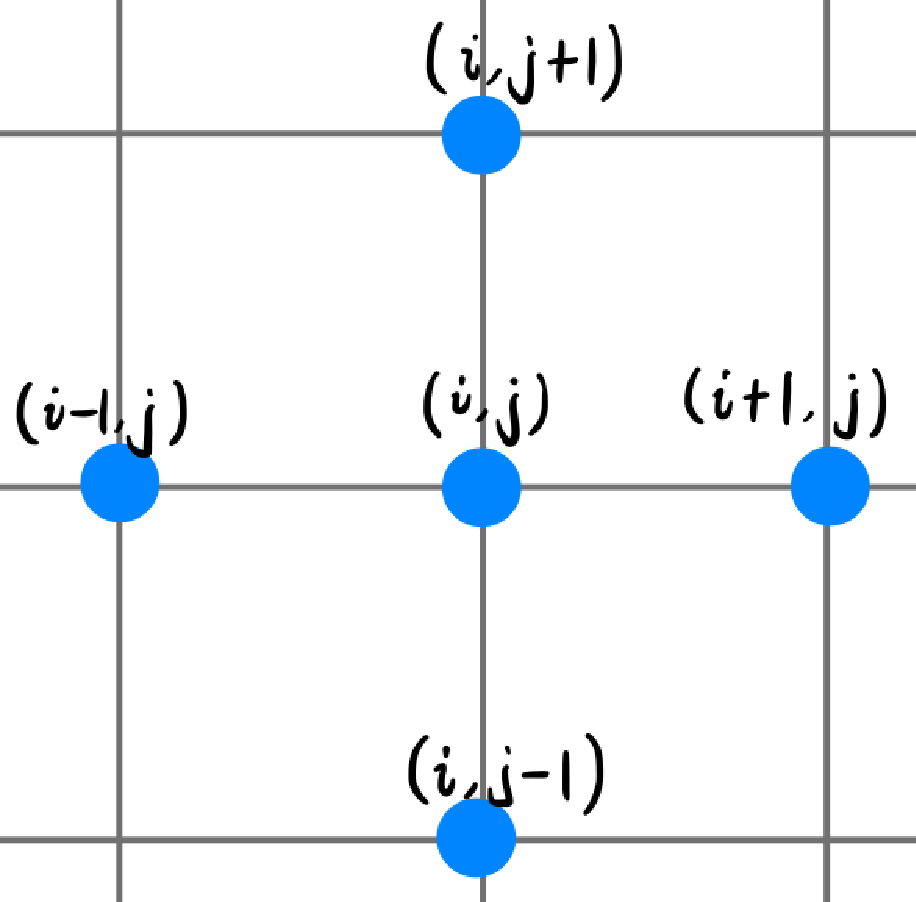
\includegraphics[width=.3\textwidth]{./figs/disc}
\end{figure}
\end{itemize}
\end{frame}

%------------------------------------------------

\subsection{Simple Random Walk method}

\begin{frame}
\frametitle{Simple Random Walk method}
\begin{figure}[htbp]
    \centering
    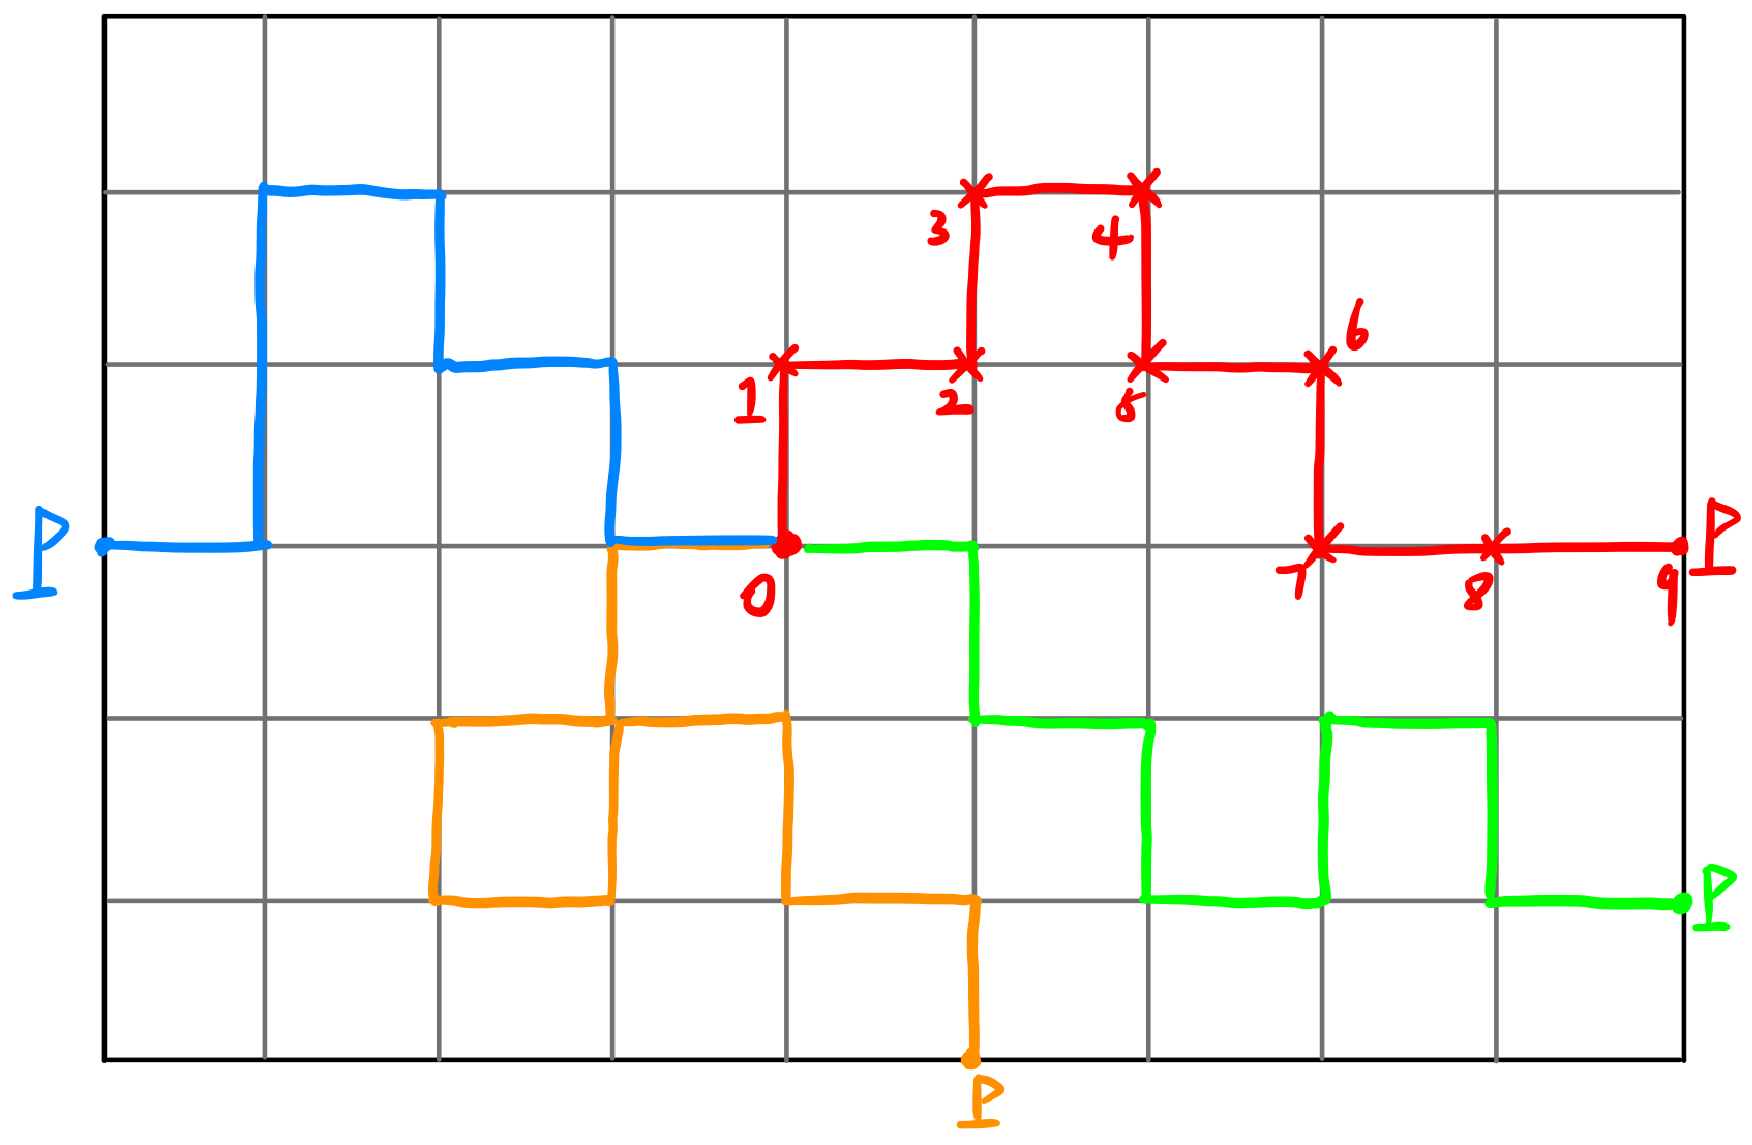
\includegraphics[width=.6\textwidth]{./figs/srw}
\end{figure}
\begin{itemize}
    \item For one random walk, we can get one estimate. Average over a large amount of estimates, we can get a precise value.
    \item The simple random walk is not very efficient, and the path doesn't really matter! We can improve it!
\end{itemize}
\end{frame}

%------------------------------------------------

\subsection{Walk on Spheres method}

\begin{frame}
\frametitle{Walk on Spheres method}
\begin{figure}[htbp]
    \centering
    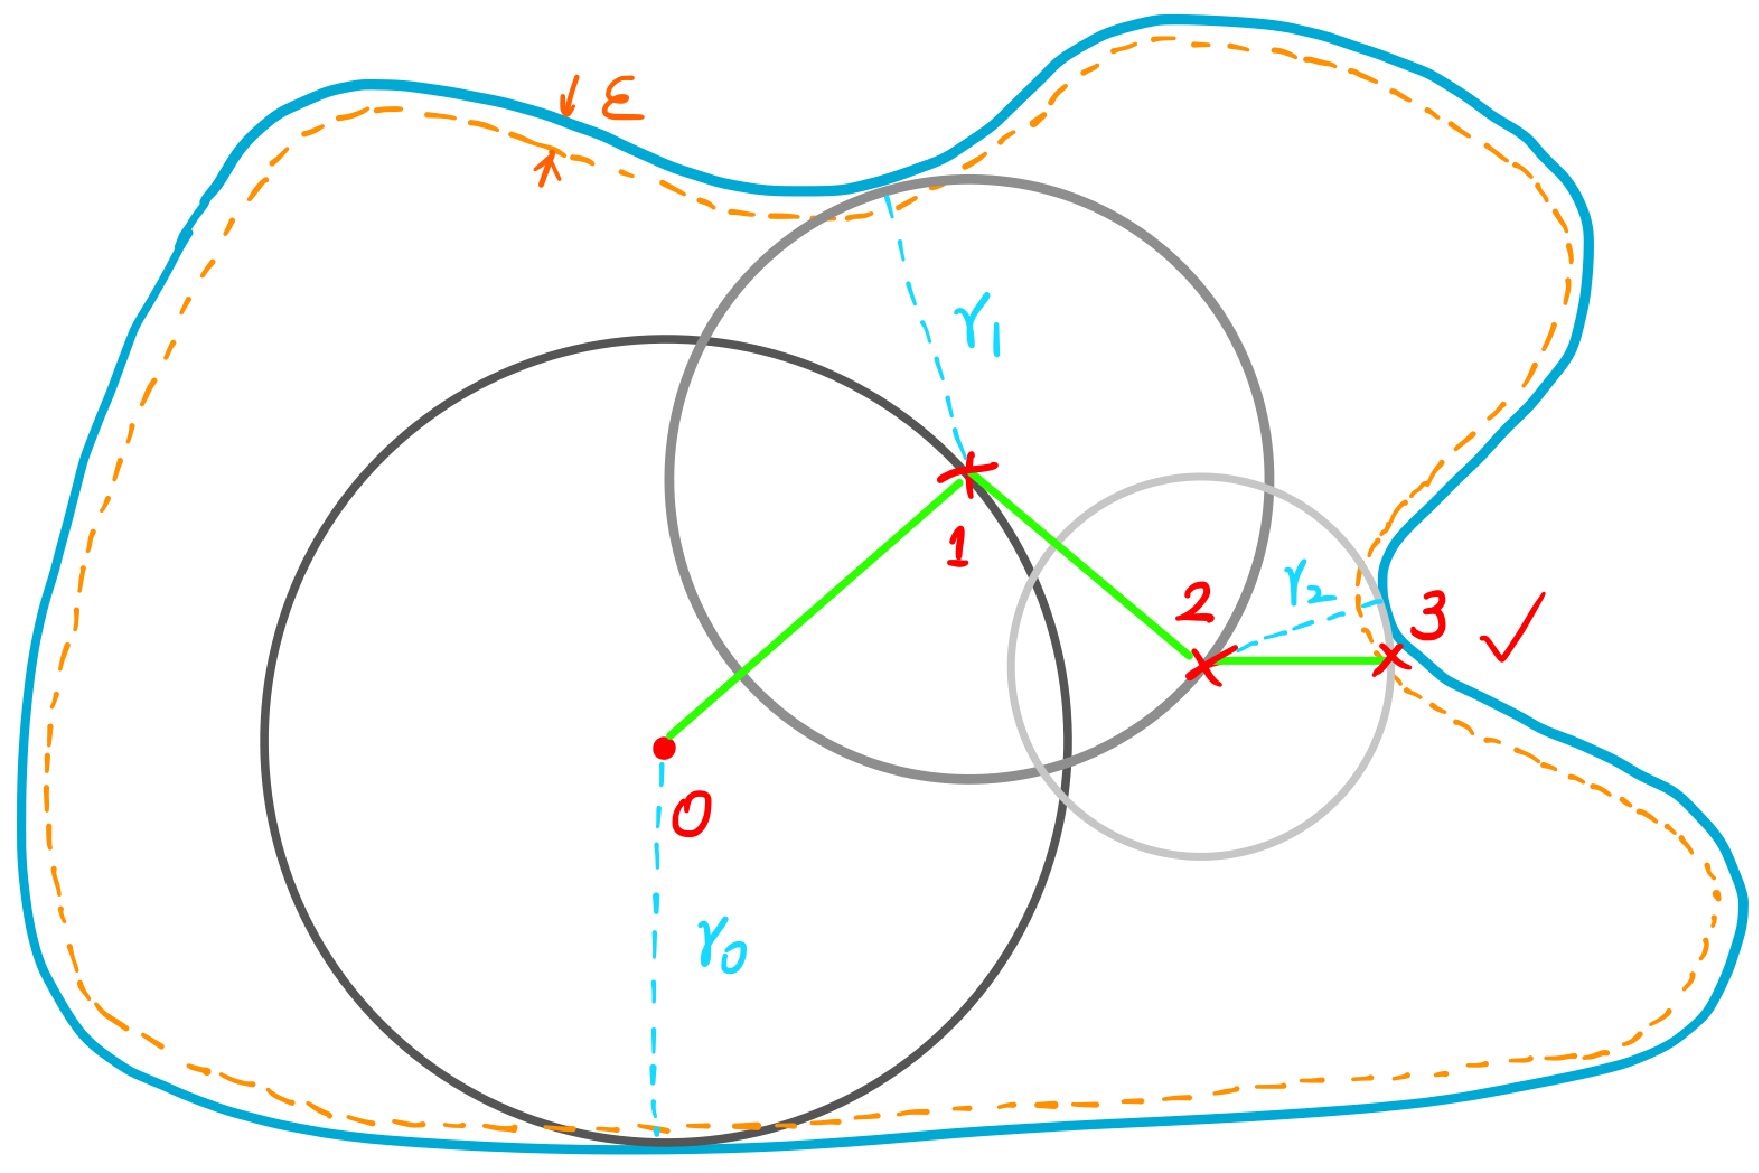
\includegraphics[width=.8\textwidth]{./figs/wos}
\end{figure}
\begin{itemize}
    \item Much faster than the Simple Random Walk method.
\end{itemize}
\end{frame}

%------------------------------------------------

\subsection{Characteristics of Monte Carlo methods}

\begin{frame}
\frametitle{Characteristics of Monte Carlo methods}
\begin{itemize}
\item \emph{Independence of points}: \textbf{The points to be evaluated are totally independent}. This makes the Monte Carlo methods \textbf{very suitable and efficient for evaluating values at certain points}.
\item \emph{Boundary \& Dimension}: It's easier for the Monte Carlo methods to \textbf{handle complex boundaries} and to be \textbf{extended to higher dimensions}.
\item \emph{Parallel Computing}: Not only different points, but also different estimates for a given point are independent. This makes the Monte Carlo methods \textbf{naturally parallel}.
\end{itemize}
\end{frame}

%------------------------------------------------

\section{Implementation \& Analysis}

%------------------------------------------------

\subsection{Parallelization}

\begin{frame}
\frametitle{Parallelization}
\begin{itemize}
\item The two straightforward ways to parallelize the program are,
\begin{enumerate}
    \item Parallelize the different estimates of one point, then average the results from different processes.
    \item Parallelize the set of points to be evaluated.
\end{enumerate}
\item For the first way,
\begin{enumerate}
    \item Allocate the estimates you want to get for every point to all available cores;
    \item Initialize the random number generator of different processes with different seeds;
    \item Wait for all the processes to finish, then collect and average the data.
\end{enumerate}
\end{itemize}
\end{frame}

%------------------------------------------------

\subsection{Square Boundary}

\begin{frame}
\frametitle{Square Boundary}
\begin{figure}[htbp]
    \centering
    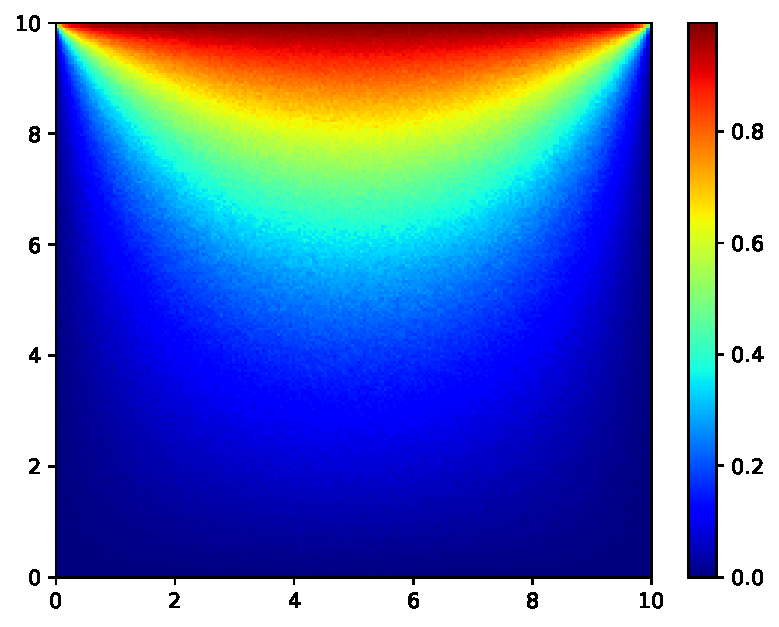
\includegraphics[width=.7\textwidth]{./figs/wos_s}
    \caption{\label{fig:wos_s} WoS method on 2D Square Boundary.}
\end{figure}
\end{frame}

%------------------------------------------------

\subsection{Circle Boundary}

\begin{frame}
\frametitle{Circle Boundary}
\begin{figure}[htbp]
    \centering
    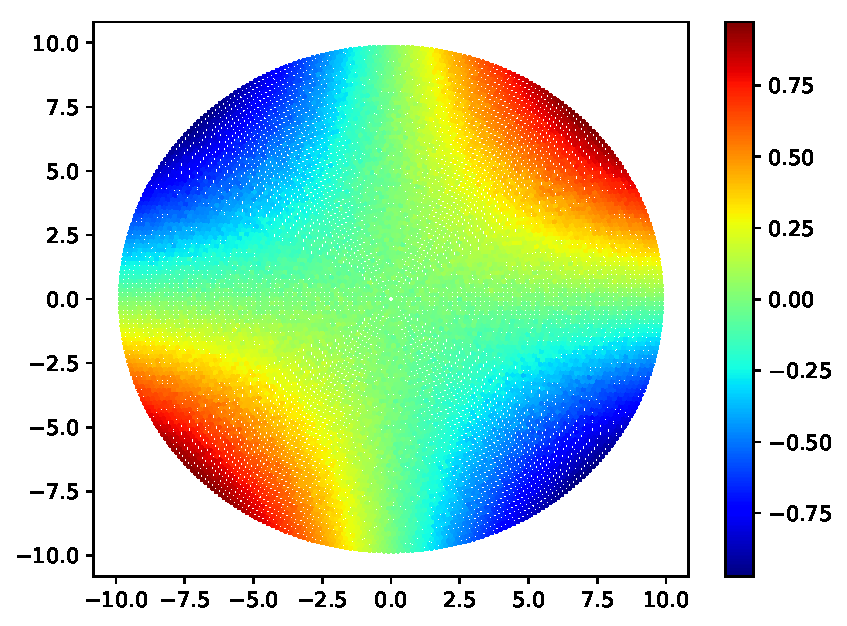
\includegraphics[width=.75\textwidth]{./figs/wos_c}
    \caption{\label{fig:wos_c} WoS method on 2D Circle Boundary.}
\end{figure}
\end{frame}

%------------------------------------------------

\subsection{Analysis of WoS method}

\begin{frame}
\frametitle{Analysis of WoS method - Running time vs. $\epsilon$}
\begin{figure}[htbp]
    \centering
    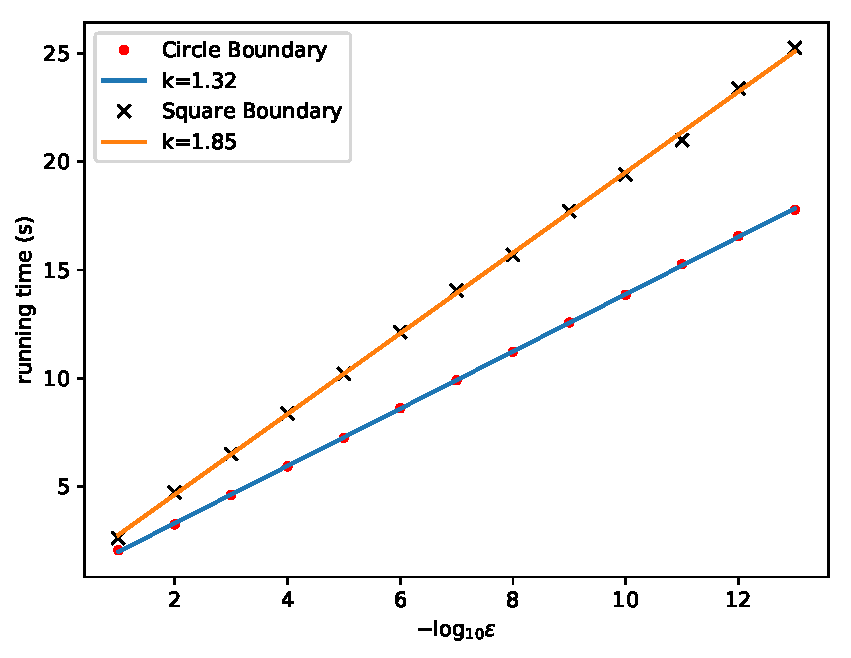
\includegraphics[width=.75\textwidth]{./figs/ep_t}
    \caption{\label{fig:ep_t} The running time - $\epsilon$ relation on both square and circle boundary.}
\end{figure}
\end{frame}

\begin{frame}
\frametitle{Analysis of WoS method - Convergence rate}

\end{frame}

%------------------------------------------------

\section{Future Work}

\begin{frame}
\frametitle{Future Work}

\end{frame}

%------------------------------------------------

\begin{frame}
\Huge{\centerline{Thank you! Questions?}}
\end{frame}

%----------------------------------------------------------------------------------------

\end{document}
